\documentclass[11pt]{article}
\usepackage[margin=1in]{geometry}
\usepackage{amsmath, amssymb, amsfonts}
\usepackage{enumitem}
\usepackage[framemethod=default]{mdframed}
\usepackage{hyperref}
\usepackage{xcolor}
\usepackage{parskip}
\usepackage{upquote}
\usepackage{graphicx}
\usepackage{float}
\usepackage{framed}
\usepackage{booktabs}
\usepackage{multirow}

\newenvironment{answer}{{\bf Answer:} \sf \begingroup\color{red}}{\endgroup}%

\definecolor{shadecolor}{gray}{0.95}

\title{CS336 Assignment 3: Writeup}
\author{Jack Le}
\date{Spring 2026}

\begin{document}
\maketitle

\section*{2.1 \quad \texttt{chinchilla\_isoflops}}

\begin{enumerate}[label=(\alph*)]
  \item Show your extrapolated compute-optimal model size, together with the $\langle C_i, N_{\text{opt}}(C_i)\rangle$ points you obtained. What is your predicted optimal model size for a budget of $10^{23}$ FLOPs? What about for $10^{24}$ FLOPs?

    \begin{answer}
      The red points are the observed $\langle C_i, N_{\text{opt}}(C_i)\rangle$ points, and the blue line is the fitted scaling law. With a budget of $10^{23}$ FLOPs, the predicted optimal model size is $5.00 \times 10^{10}$ parameters. With $10^{24}$ FLOPs, the predicted optimal model size is $1.27 \times 10^{11}$ parameters.
      \begin{figure}[H]
        \centering
        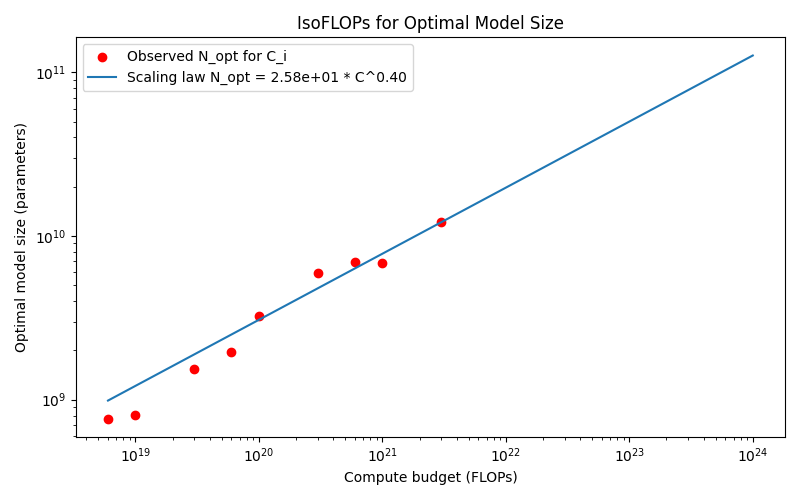
\includegraphics[width=0.8\textwidth]{figures/isoflops_model.png}
        \caption{Extrapolated compute-optimal model size}
        \label{fig:isoflops_model}
      \end{figure}

    \end{answer}

    \newpage

  \item Show your extrapolated compute-optimal dataset size, together with the $\langle C_i, D_{\text{opt}}(C_i)\rangle$ data points from the training runs. What is your predicted optimal dataset size for budgets of $10^{23}$ and $10^{24}$ FLOPs?

    \begin{answer}
      The blue points are the observed $\langle C_i, D_{\text{opt}}(C_i)\rangle$ points, and the black line is the fitted scaling law. With a budget of $10^{23}$ FLOPs, the predicted optimal dataset size is $3.37 \times 10^{11}$ tokens. With $10^{24}$ FLOPs, the predicted optimal dataset size is $1.33 \times 10^{12}$ tokens.
      \begin{figure}[H]
        \centering
        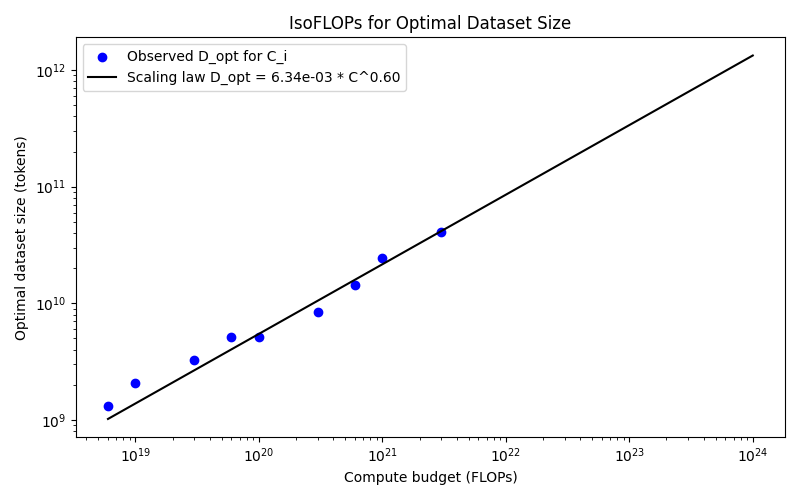
\includegraphics[width=0.8\textwidth]{figures/isoflops_dataset.png}
        \caption{Extrapolated compute-optimal dataset size}
        \label{fig:isoflops_dataset}
      \end{figure}
    \end{answer}
\end{enumerate}

\section*{3 \quad \texttt{scaling\_laws}}

\begin{answer}
\end{answer}

\end{document}